% \begin{frame}
%     \frametitle{Visualizzare ed Elaborare documenti XML}
%     \addtocounter{nframe}{1}
    
%     %\begin{center}
%     %    
\includegraphics[width=.2\textwidth]{../imgs/tei-r.pdf}
%     %\end{center}
%     %\textit{In parte già disponibili nei moduli TEI di base}

%      \begin{block}{Perché visualizzare il testo}
%     %     \emph{Per la critica testuale indispensabili i moduli}
%          \begin{itemize}
%             \item  Controllare la codifica e correggere i refusi
%              \item Assicurarsi che tutto sia stato trascritto correttamente
%              \item Mostrare il testo a persone che non conoscono XML-TEI
%              \item Disporre di una versione del lavoro fuibile
%         \end{itemize}
%      \end{block}
    
% \end{frame}

\begin{frame}
    \frametitle{Visualizzare ed Elaborare documenti XML}
    \addtocounter{nframe}{1}
    
    %\begin{center}
    %    
\includegraphics[width=.2\textwidth]{../imgs/tei-r.pdf}
    %\end{center}
    %\textit{In parte già disponibili nei moduli TEI di base}

     \begin{block}{Elemento \texttt{<xsl:template>}}
        Definisce una regola (ovvero un modello) di trasformazione per i nodi di un particolare tipo/contesto.
     \end{block}
    
\end{frame}

\begin{frame}
    \frametitle{Visualizzare ed Elaborare documenti XML}
    \addtocounter{nframe}{1}
    
    \begin{center}
        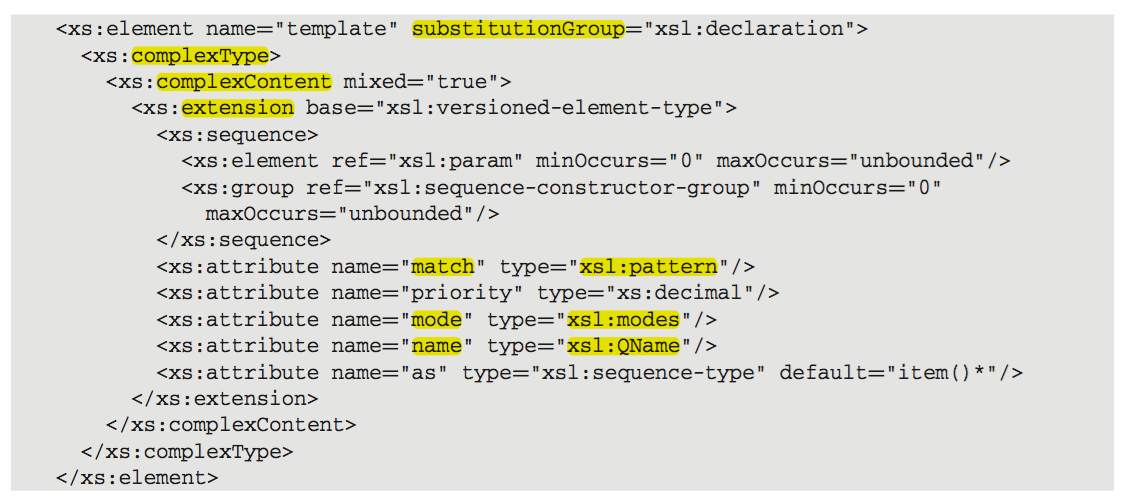
\includegraphics[width=.95\textwidth]{imgs/Schema-template.png}
    \end{center}
    %\textit{In parte già disponibili nei moduli TEI di base}

\end{frame}

\begin{frame}
    \frametitle{Visualizzare ed Elaborare documenti XML}
    \addtocounter{nframe}{1}
    
    %\begin{center}
    %    
\includegraphics[width=.2\textwidth]{../imgs/tei-r.pdf}
    %\end{center}
    %\textit{In parte già disponibili nei moduli TEI di base}

     \begin{block}{Attributi Elemento \texttt{<xsl:template>}}
    %     \emph{Per la critica testuale indispensabili i moduli}
         \begin{itemize}
             \item \textbf{name}: nome del template;
             \item \textbf{match}: pattern che indica l'elemento su cui applicare il modello;
             \item \textbf{priority}: priorità del modello;
             \item \textbf{mode}: modalità di elaborazione, che consente all'elemento di essere elaborato più volte per produrre un risultato diverso ogni volta.
        \end{itemize}
     \end{block}
    
\end{frame}


\begin{frame}
    \frametitle{Visualizzare ed Elaborare documenti XML}
    \addtocounter{nframe}{1}
    
    %\begin{center}
    %    
\includegraphics[width=.2\textwidth]{../imgs/tei-r.pdf}
    %\end{center}
    %\textit{In parte già disponibili nei moduli TEI di base}

     \begin{block}{Elemento \texttt{<xsl:template>}}
        \textit{I template XSLT possono avere due forme: }
        \begin{itemize}
            \item \textbf{"tempate rules"} che specificano una regola con pattern-matching (\texttt{<xsl:apply-templates>})
            \item \textbf{named templates} che specificano regole che possono essere chiamate esplicitamente con \texttt{<xsl:call-template>}
        \end{itemize}

     \end{block}
    
\end{frame}


%% value-of

\begin{frame}
    \frametitle{Visualizzare ed Elaborare documenti XML}
    \addtocounter{nframe}{1}
    
    %\begin{center}
    %    
\includegraphics[width=.2\textwidth]{../imgs/tei-r.pdf}
    %\end{center}
    %\textit{In parte già disponibili nei moduli TEI di base}

     \begin{block}{Elemento \texttt{<xsl:value-of>}}
        Restituisce il contenuto del nodo selezionato secondo l'espressione XPath indicata.
        \\ \textit{(Il contenuto di un elemento è costituito da tutti i caratteri che si trovano fra tag di apertura e tag di chiusura)}
     \end{block}
    
\end{frame}

\begin{frame}
    \frametitle{Visualizzare ed Elaborare documenti XML}
    \addtocounter{nframe}{1}
    
    \begin{center}
        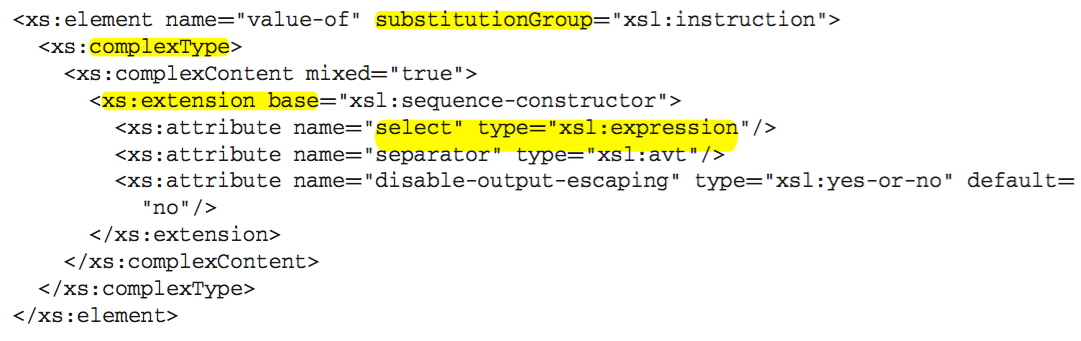
\includegraphics[width=.95\textwidth]{imgs/Schema-value-of.png}
    \end{center}
    %\textit{In parte già disponibili nei moduli TEI di base}

\end{frame}

\begin{frame}
    \frametitle{Visualizzare ed Elaborare documenti XML}
    \addtocounter{nframe}{1}
    
    %\begin{center}
    %    
\includegraphics[width=.2\textwidth]{../imgs/tei-r.pdf}
    %\end{center}
    %\textit{In parte già disponibili nei moduli TEI di base}

     \begin{block}{Attributi Elemento \texttt{<xsl:value-of>}}
    %     \emph{Per la critica testuale indispensabili i moduli}
         \begin{itemize}
             \item \textbf{select}: espressione XPath da valutare nel contesto corrente
             \item \textbf{disable-output-escaping}: default "no"; se "yes", il testo di
             output non esclude i caratteri XML dal testo
        \end{itemize}
     \end{block}
    
\end{frame}

\begin{frame}
    \frametitle{Visualizzare ed Elaborare documenti XML}
    \addtocounter{nframe}{1}
    
    %\begin{center}
    %    
\includegraphics[width=.2\textwidth]{../imgs/tei-r.pdf}
    %\end{center}
    %\textit{In parte già disponibili nei moduli TEI di base}

     \begin{block}{Esempio Elemento \texttt{<xsl:value-of>}}
        
        \texttt{<xsl:template match="fileDesc" >}
        \\\texttt{<h1>File Desc</h1>}
        \\\texttt{<p>}
            \\\texttt{<xsl:value-of select="titleStmt/title" disable-output-escaping="no" />}
        \\\texttt{</p>}
        \\\texttt{</xsl:template>}

     \end{block}
    
\end{frame}

%% Apply-templates

\begin{frame}
    \frametitle{Visualizzare ed Elaborare documenti XML}
    \addtocounter{nframe}{1}
    
    %\begin{center}
    %    
\includegraphics[width=.2\textwidth]{../imgs/tei-r.pdf}
    %\end{center}
    %\textit{In parte già disponibili nei moduli TEI di base}

     \begin{block}{Elemento \texttt{<xsl:apply-templates>}}
        Elaborare in modo ricorsivo i nodi di un documento XML a partire da un punto preciso dell'albero XML.
     \end{block}

     \begin{block}{Elemento \texttt{<xsl:apply-templates>}}
        Confronta ogni nodo presente all’interno del nodo selezionato con le template rules del foglio di stile e se viene trovata una regola applicabile questa viene applicata.
     \end{block}

\end{frame}

\begin{frame}
    \frametitle{Visualizzare ed Elaborare documenti XML}
    \addtocounter{nframe}{1}
    
    \begin{center}
        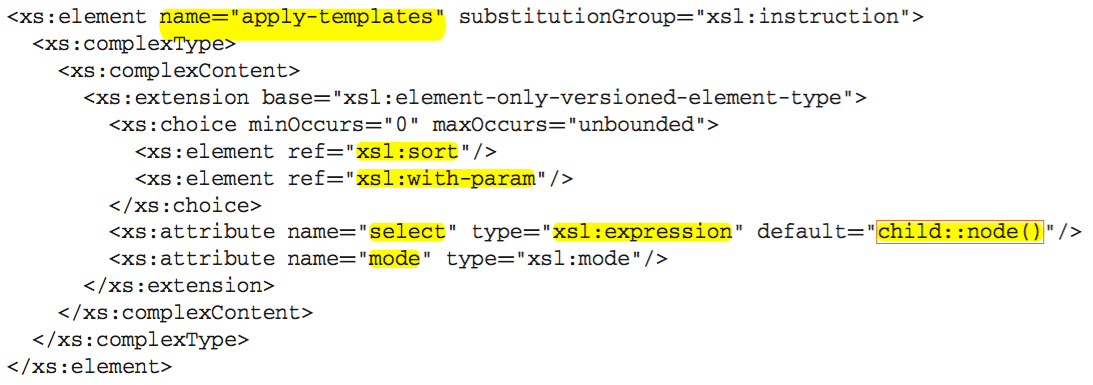
\includegraphics[width=.95\textwidth]{imgs/Schema-apply-templates.png}
    \end{center}
    %\textit{In parte già disponibili nei moduli TEI di base}

\end{frame}

\begin{frame}
    \frametitle{Visualizzare ed Elaborare documenti XML}
    \addtocounter{nframe}{1}
    
    %\begin{center}
    %    
\includegraphics[width=.2\textwidth]{../imgs/tei-r.pdf}
    %\end{center}
    %\textit{In parte già disponibili nei moduli TEI di base}

     \begin{block}{Attributi Elemento \texttt{<xsl:apply-templates>}}
    %     \emph{Per la critica testuale indispensabili i moduli}
         \begin{itemize}
             \item \textbf{select}: espressione XPath
             \item \textbf{mode}: modalità di elaborazione
        \end{itemize}
     \end{block}
    
\end{frame}

\begin{frame}
    \frametitle{Visualizzare ed Elaborare documenti XML}
    \addtocounter{nframe}{1}
    
    %\begin{center}
    %    
\includegraphics[width=.2\textwidth]{../imgs/tei-r.pdf}
    %\end{center}
    %\textit{In parte già disponibili nei moduli TEI di base}

     \begin{block}{Esempio Elemento \texttt{<xsl:apply-templates>}}
        
        \texttt{<xsl:template match="/" >}
        \\\texttt{<html><head>}
        \\\texttt{<title><xsl:value-of select="TEI/teiHeader/fileDesc/title"/></title>}
        \\\texttt{</head><body><div><span>1.</span>}
        \\\texttt{<xsl:apply-templates select="TEI/teiHeader/fileDesc" />}
        \\\texttt{</div></body></html></xsl:template>}

     \end{block}
    
\end{frame}


%% xsl:for-each

\begin{frame}
    \frametitle{Visualizzare ed Elaborare documenti XML}
    \addtocounter{nframe}{1}
    
    %\begin{center}
    %    
\includegraphics[width=.2\textwidth]{../imgs/tei-r.pdf}
    %\end{center}
    %\textit{In parte già disponibili nei moduli TEI di base}

     \begin{block}{Elemento \texttt{<xsl:for-each>}}
        Se sono presenti più nodi con lo stesso nome (e manca un’istruzione ricorsiva precedente) \texttt{<xsl:value-of>} restituisce il valore del primo che incontra.
     \end{block}

     \begin{block}{Elemento \texttt{<xsl:for-each>}}
        è quindi possibile usare l’istruzione \texttt{<xsl:for-each>} e applicare un’istruzione \texttt{<xsl:value-of>} a tutti i nodi identificati dalla regola.
     \end{block}

\end{frame}

\begin{frame}
    \frametitle{Visualizzare ed Elaborare documenti XML}
    \addtocounter{nframe}{1}
    
    \begin{center}
        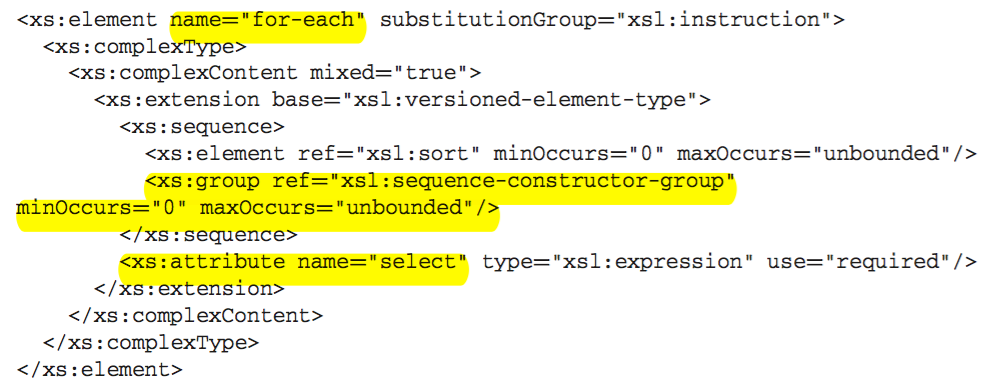
\includegraphics[width=.95\textwidth]{imgs/Schema-for-each.png}
    \end{center}
    %\textit{In parte già disponibili nei moduli TEI di base}

\end{frame}

\begin{frame}
    \frametitle{Visualizzare ed Elaborare documenti XML}
    \addtocounter{nframe}{1}
    
    %\begin{center}
    %    
\includegraphics[width=.2\textwidth]{../imgs/tei-r.pdf}
    %\end{center}
    %\textit{In parte già disponibili nei moduli TEI di base}

     \begin{block}{Attributi Elemento \texttt{<xsl:for-each>}}
    %     \emph{Per la critica testuale indispensabili i moduli}
         \begin{itemize}
             \item \textbf{select}: espressione XPath
        \end{itemize}
     \end{block}
    
\end{frame}

\begin{frame}
    \frametitle{Visualizzare ed Elaborare documenti XML}
    \addtocounter{nframe}{1}
    
    %\begin{center}
    %    
\includegraphics[width=.2\textwidth]{../imgs/tei-r.pdf}
    %\end{center}
    %\textit{In parte già disponibili nei moduli TEI di base}

     \begin{block}{Esempio Elemento \texttt{<xsl:for-each>}}
        
        \texttt{<xsl:template match="/" >}
        \\\texttt{<html><head>}
        \\\texttt{<title><xsl:value-of select="TEI/teiHeader/fileDesc/title"/></title>}
        \\\texttt{</head><body><div>}
        \\\texttt{<xsl:for-each select="//div" >}
        \\\texttt{<div><xsl:value-of select="./p" /></div>}
        \\\texttt{</xsl:for-each></div></body></html>}
     \end{block}
    
\end{frame}


%% xsl:text


\begin{frame}
    \frametitle{Visualizzare ed Elaborare documenti XML}
    \addtocounter{nframe}{1}
    
    %\begin{center}
    %    
\includegraphics[width=.2\textwidth]{../imgs/tei-r.pdf}
    %\end{center}
    %\textit{In parte già disponibili nei moduli TEI di base}

     \begin{block}{Elemento \texttt{<xsl:text>}}
        Permette di inserire una stringa di testo nell’albero di output.
     \end{block}

     \begin{block}{Elemento \texttt{<xsl:text>}}
        Molto utile se si è deciso di eliminare tutti gli spazi e gli a capo.
     \end{block}
     

\end{frame}

\begin{frame}
    \frametitle{Visualizzare ed Elaborare documenti XML}
    \addtocounter{nframe}{1}
    
    \begin{center}
        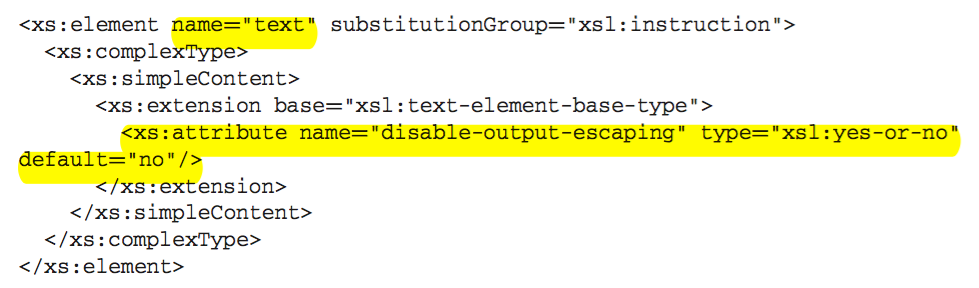
\includegraphics[width=.95\textwidth]{imgs/Schema-text.png}
    \end{center}
    %\textit{In parte già disponibili nei moduli TEI di base}

\end{frame}

\begin{frame}
    \frametitle{Visualizzare ed Elaborare documenti XML}
    \addtocounter{nframe}{1}
    
    %\begin{center}
    %    
\includegraphics[width=.2\textwidth]{../imgs/tei-r.pdf}
    %\end{center}
    %\textit{In parte già disponibili nei moduli TEI di base}

     \begin{block}{Attributi Elemento \texttt{<xsl:text>}}
    %     \emph{Per la critica testuale indispensabili i moduli}
         \begin{itemize}
             \item \textbf{disable-output-escaping}: se "yes", consente di copiare i caratteri di marcatura non identificati nell'albero di output.
        \end{itemize}
     \end{block}
    
\end{frame}

\begin{frame}
    \frametitle{Visualizzare ed Elaborare documenti XML}
    \addtocounter{nframe}{1}
    
    %\begin{center}
    %    
\includegraphics[width=.2\textwidth]{../imgs/tei-r.pdf}
    %\end{center}
    %\textit{In parte già disponibili nei moduli TEI di base}

     \begin{block}{Esempio Elemento \texttt{<xsl:text>}}
        
        \texttt{<xsl:for-each select="\$attr" >}
        \\\texttt{<xsl:value-of select="concat('[',position(),']',current())" />}
        \\\texttt{<xsl:text>\&\#32;</xsl:text>}
        \\\texttt{</xsl:for-each>}

     \end{block}

\end{frame}

%% if
\begin{frame}
    \frametitle{Visualizzare ed Elaborare documenti XML}
    \addtocounter{nframe}{1}
    
    %\begin{center}
    %    
\includegraphics[width=.2\textwidth]{../imgs/tei-r.pdf}
    %\end{center}
    %\textit{In parte già disponibili nei moduli TEI di base}

     \begin{block}{Elemento \texttt{<xsl:if>}}
        Identifica una condizione semplice: la regola viene eseguita soltanto se la condizione viene soddisfatta.
     \end{block}

\end{frame}

\begin{frame}
    \frametitle{Visualizzare ed Elaborare documenti XML}
    \addtocounter{nframe}{1}
    
    \begin{center}
        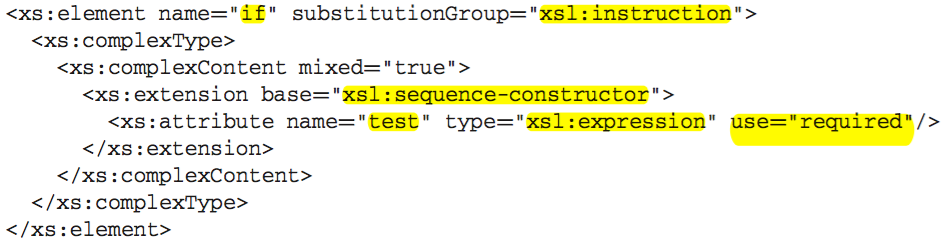
\includegraphics[width=.95\textwidth]{imgs/Schema-if.png}
    \end{center}
    %\textit{In parte già disponibili nei moduli TEI di base}

\end{frame}

\begin{frame}
    \frametitle{Visualizzare ed Elaborare documenti XML}
    \addtocounter{nframe}{1}
    
    %\begin{center}
    %    
\includegraphics[width=.2\textwidth]{../imgs/tei-r.pdf}
    %\end{center}
    %\textit{In parte già disponibili nei moduli TEI di base}

     \begin{block}{Attributi Elemento \texttt{<xsl:if>}}
    %     \emph{Per la critica testuale indispensabili i moduli}
         \begin{itemize}
             \item \textbf{test}: l’espressione di test. Se restituisce true, il contenuto di \texttt{<xsl:if>} viene valutato e inserito nell’albero di output; altrimenti viene ignorato
        \end{itemize}
     \end{block}
    
\end{frame}

\begin{frame}
    \frametitle{Visualizzare ed Elaborare documenti XML}
    \addtocounter{nframe}{1}
    
    %\begin{center}
    %    
\includegraphics[width=.2\textwidth]{../imgs/tei-r.pdf}
    %\end{center}
    %\textit{In parte già disponibili nei moduli TEI di base}

     \begin{block}{Esempio Elemento \texttt{<xsl:if>}}
        
        \texttt{<xsl:if test="@n='23'" >...</xsl:if>}
        \\\texttt{<xsl:if test="title[@level='m']" >...</xsl:if>}
        \\\texttt{<xsl:if test="count(verse) > 3" >...</xsl:if>}
        \\\texttt{}

     \end{block}

\end{frame}


%% xsl:choose
\begin{frame}
    \frametitle{Visualizzare ed Elaborare documenti XML}
    \addtocounter{nframe}{1}
    
    %\begin{center}
    %    
\includegraphics[width=.2\textwidth]{../imgs/tei-r.pdf}
    %\end{center}
    %\textit{In parte già disponibili nei moduli TEI di base}

     \begin{block}{Elemento \texttt{<xsl:choose>}}
        Permette di definire condizioni multiple tra cui scegliere.
     \end{block}

     \begin{block}{Elemento \texttt{<xsl:choose>}}
        Il content model di \textit{choose} prevede uno o più elementi \texttt{<xsl:when>} e opzionalmente l'elemento \texttt{<xsl:otherwise>}.
     \end{block}

\end{frame}

\begin{frame}
    \frametitle{Visualizzare ed Elaborare documenti XML}
    \addtocounter{nframe}{1}
    
    \begin{center}
        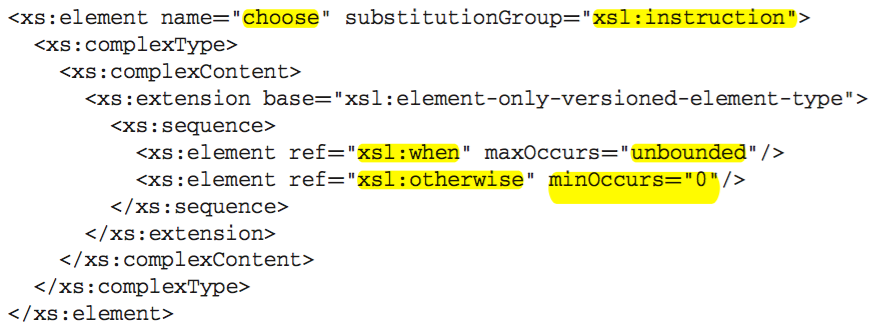
\includegraphics[width=.95\textwidth]{imgs/Schema-choose.png}
    \end{center}
    %\textit{In parte già disponibili nei moduli TEI di base}

\end{frame}

% \begin{frame}
%     \frametitle{Visualizzare ed Elaborare documenti XML}
%     \addtocounter{nframe}{1}
    
%     %\begin{center}
%     %    
\includegraphics[width=.2\textwidth]{../imgs/tei-r.pdf}
%     %\end{center}
%     %\textit{In parte già disponibili nei moduli TEI di base}

%      \begin{block}{Attributi Elemento \texttt{<xsl:if>}}
%     %     \emph{Per la critica testuale indispensabili i moduli}
%          \begin{itemize}
%              \item \textbf{test}: l’espressione di test. Se restituisce true, il contenuto di \texttt{<xsl:if>} viene valutato e inserito nell’albero di output; altrimenti viene ignorato
%         \end{itemize}
%      \end{block}
    
% \end{frame}

\begin{frame}
    \frametitle{Visualizzare ed Elaborare documenti XML}
    \addtocounter{nframe}{1}
    
    %\begin{center}
    %    
\includegraphics[width=.2\textwidth]{../imgs/tei-r.pdf}
    %\end{center}
    %\textit{In parte già disponibili nei moduli TEI di base}

     \begin{block}{Esempio Elemento \texttt{<xsl:choose>}}
        
        \texttt{<xsl:template match="tei:title" >}
        \\\texttt{<xsl:choose>}
        \\\texttt{<xsl:when test="@level = 'm' or @level = 'u'" >}
        \\\texttt{<i><xsl:apply-templates/>. </i> </xsl:when>}
        \\\texttt{<xsl:when test="@level = 'j'" >}
        \\\texttt{<i><xsl:apply-templates/></i>}
        \\\texttt{</xsl:when>}
        \\\texttt{<xsl:otherwise>}
        \\\texttt{<i><xsl:apply-templates/></i></xsl:otherwise>}
        \\\texttt{</xsl:choose></xsl:template>}
     \end{block}

\end{frame}

% xsl:sort

\begin{frame}
    \frametitle{Visualizzare ed Elaborare documenti XML}
    \addtocounter{nframe}{1}
    
    %\begin{center}
    %    
\includegraphics[width=.2\textwidth]{../imgs/tei-r.pdf}
    %\end{center}
    %\textit{In parte già disponibili nei moduli TEI di base}

     \begin{block}{Elemento \texttt{<xsl:sort>}}
        Permette di riorganizzare l’ordine in cui vengono scritti i nodi nell’albero di output.
     \end{block}

     \begin{block}{Elemento \texttt{<xsl:sort>}}
        Deve comparire all’interno di un’istruzione \texttt{<xsl:apply-templates>} o \texttt{<xsl:for-each>}.
     \end{block}

\end{frame}

\begin{frame}
    \frametitle{Visualizzare ed Elaborare documenti XML}
    \addtocounter{nframe}{1}
    
    \begin{center}
        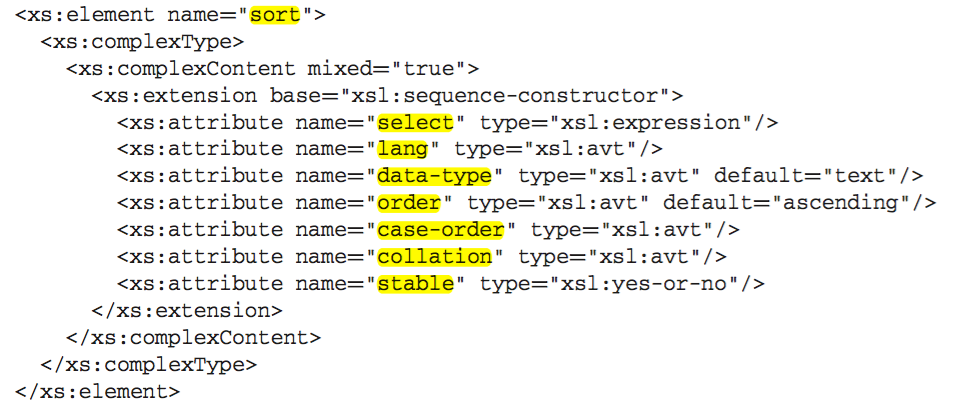
\includegraphics[width=.95\textwidth]{imgs/Schema-sort.png}
    \end{center}
    %\textit{In parte già disponibili nei moduli TEI di base}

\end{frame}

\begin{frame}
    \frametitle{Visualizzare ed Elaborare documenti XML}
    \addtocounter{nframe}{1}
    
    %\begin{center}
    %    
\includegraphics[width=.2\textwidth]{../imgs/tei-r.pdf}
    %\end{center}
    %\textit{In parte già disponibili nei moduli TEI di base}

     \begin{block}{Attributi Elemento \texttt{<xsl:sort>}}
    %     \emph{Per la critica testuale indispensabili i moduli}
         \begin{itemize}
             \item \textbf{select}: espressione XPath per individuare gli elementi in base ai quali effettuare l’ordinamento.
             \item \textbf{lang}: linguaggio utilizzato per l’ordinamento.
             \item \textbf{data-type}: il tipo degli elementi rispetto ai quali stiamo effettuando l’ordinamento.
             \item \textbf{order}: ordinamento crescente (ascending) o discendente (descending)
             \item \textbf{case-order}: indica se dare precedenza ai caratteri minuscoli (lower-first) o maiuscoli (upper-first)
        \end{itemize}
     \end{block}
    
\end{frame}

\begin{frame}
    \frametitle{Visualizzare ed Elaborare documenti XML}
    \addtocounter{nframe}{1}
    
    %\begin{center}
    %    
\includegraphics[width=.2\textwidth]{../imgs/tei-r.pdf}
    %\end{center}
    %\textit{In parte già disponibili nei moduli TEI di base}

     \begin{block}{Esempio Elemento \texttt{<xsl:sort>}}
        
        \texttt{<div><ul><xsl:for-each select="TEI/text/body/div" >}
        \\\texttt{<xsl:sort select="@n" data-type="number" order="descending" />}
        \\\texttt{<li><xsl:value-of select="@n" />}
        \\\texttt{<xsl:text>|</xsl:text>}
        \\\texttt{<xsl:value-of select="current()" /></li>}
        \\\texttt{</xsl:for-each></ul></div>}

     \end{block}
\end{frame}

%% xsl:variable

\begin{frame}
    \frametitle{Visualizzare ed Elaborare documenti XML}
    \addtocounter{nframe}{1}
    
    %\begin{center}
    %    
\includegraphics[width=.2\textwidth]{../imgs/tei-r.pdf}
    %\end{center}
    %\textit{In parte già disponibili nei moduli TEI di base}

     \begin{block}{Elemento \texttt{<xsl:variable>}}
        Permette di definire una variabile, ovvero una posizione di memorizzazione denominata in un modo personalizzato, che contiene i risultati di una espressione valutata a runtime.
     \end{block}

     \begin{block}{Elemento \texttt{<xsl:variable>}}
        L’accesso ad una variabile avviene anteponendo il carattere \$ al nome della variabile (es.: \$unaVariabile).
     \end{block}

\end{frame}

\begin{frame}
    \frametitle{Visualizzare ed Elaborare documenti XML}
    \addtocounter{nframe}{1}
    
    \begin{center}
        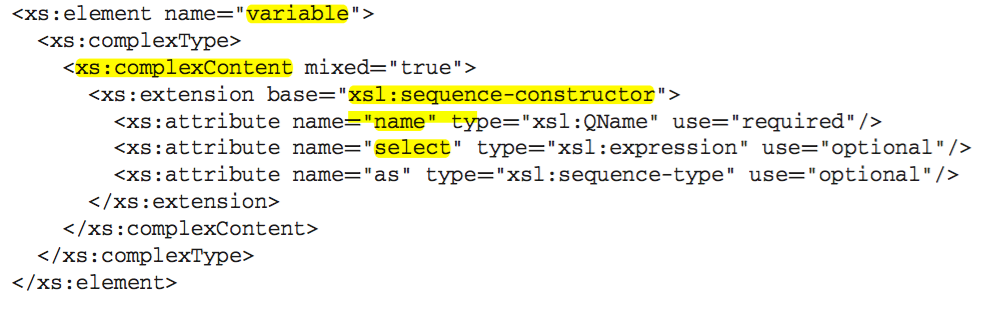
\includegraphics[width=.95\textwidth]{imgs/Schema-variable.png}
    \end{center}
    %\textit{In parte già disponibili nei moduli TEI di base}

\end{frame}

\begin{frame}
    \frametitle{Visualizzare ed Elaborare documenti XML}
    \addtocounter{nframe}{1}
    
    %\begin{center}
    %    
\includegraphics[width=.2\textwidth]{../imgs/tei-r.pdf}
    %\end{center}
    %\textit{In parte già disponibili nei moduli TEI di base}

     \begin{block}{Attributi Elemento \texttt{<xsl:variable>}}
    %     \emph{Per la critica testuale indispensabili i moduli}
         \begin{itemize}
             \item \textbf{name}: nome della variabile.
             \item \textbf{select}: seleziona il contenuto della variabile, se presente; altrimenti come contenuto viene usato il contenuto dell’istruzione 
        \end{itemize}
     \end{block}
    
\end{frame}

\begin{frame}
    \frametitle{Visualizzare ed Elaborare documenti XML}
    \addtocounter{nframe}{1}
    
    %\begin{center}
    %    
\includegraphics[width=.2\textwidth]{../imgs/tei-r.pdf}
    %\end{center}
    %\textit{In parte già disponibili nei moduli TEI di base}
    \textbf{La definizione di variabili può assumere tre distinte forme:}

     \begin{block}{Esempio Elemento \texttt{<xsl:variable>}}
        \begin{itemize}
            \item creazione di una variabile il cui valore è una stringa vuota
            \item creazione di una variabile avente valore definito dall'attributo select
            \item creazione mediante inclusione di contenuto nel corpo dell'elemento
        \end{itemize}
     \end{block}
\end{frame}

\begin{frame}
    \frametitle{Visualizzare ed Elaborare documenti XML}
    \addtocounter{nframe}{1}
    
    %\begin{center}
    %    
\includegraphics[width=.2\textwidth]{../imgs/tei-r.pdf}
    %\end{center}
    %\textit{In parte già disponibili nei moduli TEI di base}
    \textbf{La definizione di variabili può assumere tre distinte forme:}

     \begin{block}{Esempio Elemento \texttt{<xsl:variable>}}
        \begin{itemize}
            \item \texttt{<xsl:variable name="myVar" />}
            \item \texttt{<xsl:variable name="myVar" select="150" />}
            \item \texttt{<xsl:variable name="myVar" >}
            \item[] \texttt{<xs:value-of select="@n"/>}
            \item[] \texttt{</xsl:variable>}
        \end{itemize}

     \end{block}
\end{frame}

%% xsl:param

\begin{frame}
    \frametitle{Visualizzare ed Elaborare documenti XML}
    \addtocounter{nframe}{1}
    
    %\begin{center}
    %    
\includegraphics[width=.2\textwidth]{../imgs/tei-r.pdf}
    %\end{center}
    %\textit{In parte già disponibili nei moduli TEI di base}

     \begin{block}{Elemento \texttt{<xsl:param>}}
        E' simile ad una \texttt{<xsl:variable>}, ma il suo valore può essere modificato in base al modo in cui il template viene chiamato o dal foglio di stile stesso.
     \end{block}

     \begin{block}{Elemento \texttt{<xsl:param>}}
        Può essere inserita come primo figlio di un \texttt{<xsl:template>}
     \end{block}

\end{frame}

\begin{frame}
    \frametitle{Visualizzare ed Elaborare documenti XML}
    \addtocounter{nframe}{1}
    
    \begin{center}
        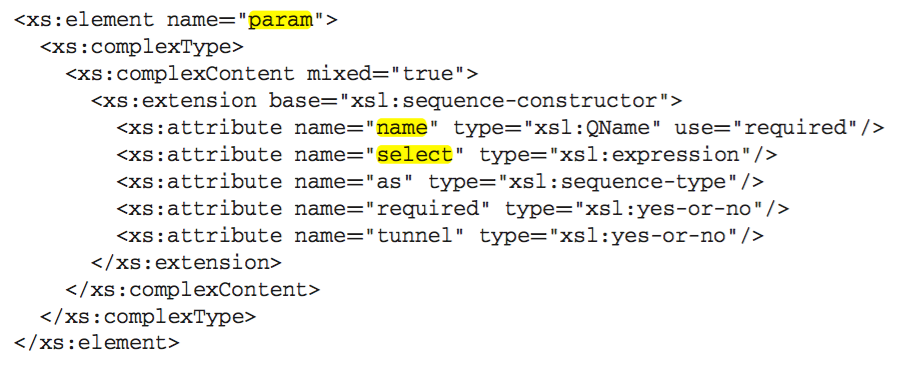
\includegraphics[width=.95\textwidth]{imgs/Schema-param.png}
    \end{center}
    %\textit{In parte già disponibili nei moduli TEI di base}

\end{frame}

\begin{frame}
    \frametitle{Visualizzare ed Elaborare documenti XML}
    \addtocounter{nframe}{1}
    
    %\begin{center}
    %    
\includegraphics[width=.2\textwidth]{../imgs/tei-r.pdf}
    %\end{center}
    %\textit{In parte già disponibili nei moduli TEI di base}

     \begin{block}{Attributi Elemento \texttt{<xsl:param>}}
    %     \emph{Per la critica testuale indispensabili i moduli}
         \begin{itemize}
             \item \textbf{name}: nome della variabile.
             \item \textbf{select}: seleziona il contenuto della variabile, se presente; altrimenti come contenuto viene usato il contenuto dell’istruzione stessa
        \end{itemize}
     \end{block}
    
\end{frame}

\begin{frame}
    \frametitle{Visualizzare ed Elaborare documenti XML}
    \addtocounter{nframe}{1}
    
    %\begin{center}
    %    
\includegraphics[width=.2\textwidth]{../imgs/tei-r.pdf}
    %\end{center}
    %\textit{In parte già disponibili nei moduli TEI di base}

     \begin{block}{Esempio Elemento \texttt{<xsl:param>}}
        
        \texttt{<xsl:template name="body" >}
        \\\texttt{<xsl:param name="style" >color:blue</xsl:param>}
        \\\texttt{<div><xsl:attribute name="style" >}
        \\\texttt{<xsl:value-of select="\$style" />}
        \\\texttt{</xsl:attribute>}
        \\\texttt{<xsl:value-of select="." /></div>}
        \\\texttt{</xsl:template>}

     \end{block}
\end{frame}

%% xsl:call-template
\begin{frame}
    \frametitle{Visualizzare ed Elaborare documenti XML}
    \addtocounter{nframe}{1}
    
    %\begin{center}
    %    
\includegraphics[width=.2\textwidth]{../imgs/tei-r.pdf}
    %\end{center}
    %\textit{In parte già disponibili nei moduli TEI di base}

     \begin{block}{Elemento \texttt{<xsl:call-template>}}
        Dopo aver assegnato un nome ad un template, è possibile richiamarlo con l’istruzione \texttt{<xsl:call-template>}.
     \end{block}

     \begin{block}{Elemento \texttt{<xsl:call-template>}}
        Per invocare un template passando dei parametri è possibile utilizzare l’elemento \texttt{<xsl:with-param>} nel corpo dell’elemento \texttt{<xsl:call-template>} o \texttt{<xsl:apply-templates>} indicando il nome del parametro ed il valore.
     \end{block}

\end{frame}

\begin{frame}
    \frametitle{Visualizzare ed Elaborare documenti XML}
    \addtocounter{nframe}{1}
    
    \begin{center}
        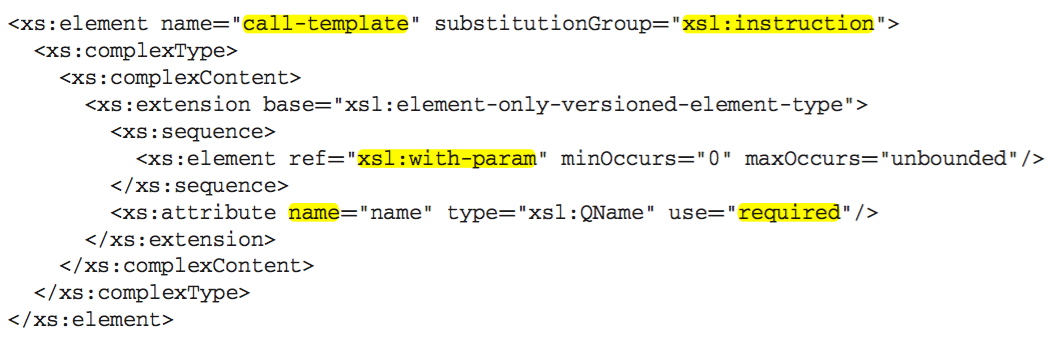
\includegraphics[width=.95\textwidth]{imgs/Schema-call-template.png}
    \end{center}
    %\textit{In parte già disponibili nei moduli TEI di base}

\end{frame}

\begin{frame}
    \frametitle{Visualizzare ed Elaborare documenti XML}
    \addtocounter{nframe}{1}
    
    %\begin{center}
    %    
\includegraphics[width=.2\textwidth]{../imgs/tei-r.pdf}
    %\end{center}
    %\textit{In parte già disponibili nei moduli TEI di base}

     \begin{block}{Attributi Elemento \texttt{<xsl:call-template>}}
    %     \emph{Per la critica testuale indispensabili i moduli}
         \begin{itemize}
             \item \textbf{name}: il nome del template da richiamare. Il foglio di stile deve necessariamente contenere un \texttt{<xsl:template>} con tale nome specificato
        \end{itemize}
     \end{block}
    
\end{frame}

\begin{frame}
    \frametitle{Visualizzare ed Elaborare documenti XML}
    \addtocounter{nframe}{1}
    
    %\begin{center}
    %    
\includegraphics[width=.2\textwidth]{../imgs/tei-r.pdf}
    %\end{center}
    %\textit{In parte già disponibili nei moduli TEI di base}

     \begin{block}{Esempio Elemento \texttt{<xsl:call-template>}}
        
        \texttt{<body>}
        \\\texttt{<xsl:call-template name="body" >}
        \\\texttt{<xsl:with-param name="style" >}
        \\\texttt{color:red </xsl:with-param>}
        \\\texttt{</xsl:call-template></body>}

     \end{block}
\end{frame}


%% xsl:element
\begin{frame}
    \frametitle{Visualizzare ed Elaborare documenti XML}
    \addtocounter{nframe}{1}
    
    %\begin{center}
    %    
\includegraphics[width=.2\textwidth]{../imgs/tei-r.pdf}
    %\end{center}
    %\textit{In parte già disponibili nei moduli TEI di base}

     \begin{block}{Elemento \texttt{<xsl:element>}}
        Per creare elementi è possibile utilizzare l'istruzione \texttt{<xsl:element>}.
     \end{block}

\end{frame}

\begin{frame}
    \frametitle{Visualizzare ed Elaborare documenti XML}
    \addtocounter{nframe}{1}
    
    \begin{center}
        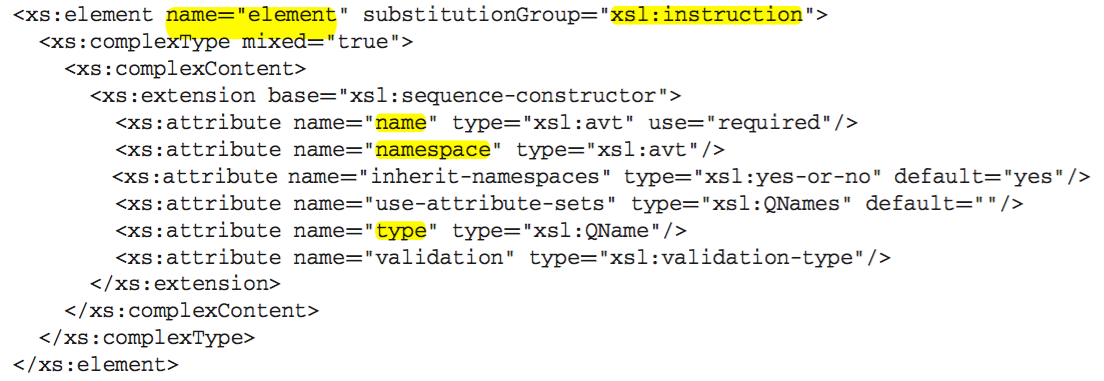
\includegraphics[width=.95\textwidth]{imgs/Schema-element.png}
    \end{center}
    %\textit{In parte già disponibili nei moduli TEI di base}

\end{frame}

\begin{frame}
    \frametitle{Visualizzare ed Elaborare documenti XML}
    \addtocounter{nframe}{1}
    
    \begin{center}
        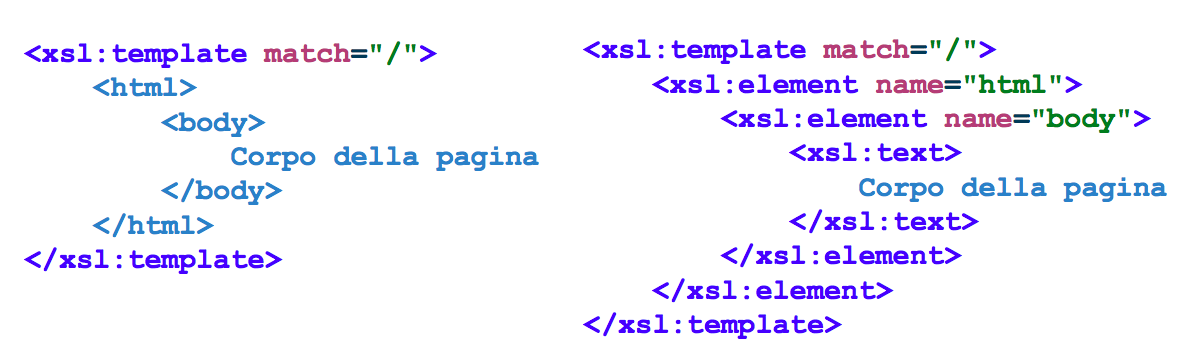
\includegraphics[width=.95\textwidth]{imgs/element-example.png}
    \end{center}
    %\textit{In parte già disponibili nei moduli TEI di base}

\end{frame}


%% xsl:attribute

\begin{frame}
    \frametitle{Visualizzare ed Elaborare documenti XML}
    \addtocounter{nframe}{1}
    
    %\begin{center}
    %    
\includegraphics[width=.2\textwidth]{../imgs/tei-r.pdf}
    %\end{center}
    %\textit{In parte già disponibili nei moduli TEI di base}

     \begin{block}{Elemento \texttt{<xsl:attribute>}}
        E' possibile creare attributi utilizzando l’elemento \texttt{<xsl:attribute>} ed indicando negli attributi \textit{name} e \textit{namespace} (opzionale) il nome e il namespace di appartenenza dell’attributo.
     \end{block}

\end{frame}

\begin{frame}
    \frametitle{Visualizzare ed Elaborare documenti XML}
    \addtocounter{nframe}{1}
    
    \begin{center}
        \includegraphics[width=.95\textwidth]{imgs/Schema-attributo.png}
    \end{center}
    %\textit{In parte già disponibili nei moduli TEI di base}

\end{frame}


\begin{frame}
    \frametitle{Visualizzare ed Elaborare documenti XML}
    \addtocounter{nframe}{1}
    
    %\begin{center}
    %    \includegraphics[width=.2\textwidth]{../imgs/tei-r.pdf}
    %\end{center}
    %\textit{In parte già disponibili nei moduli TEI di base}

     \begin{block}{Esempio Elemento \texttt{<xsl:attribute>}}
        
        \texttt{<xsl:element name="div" >}
        \\\texttt{<xsl:attribute name="id" >}
        \\\texttt{<xsl:value-of select="@id"/>}
        \\\texttt{</xsl:attribute>}
        \\\texttt{</xsl:element>}

     \end{block}
\end{frame}


%% xsl:comment
\begin{frame}
    \frametitle{Visualizzare ed Elaborare documenti XML}
    \addtocounter{nframe}{1}
    
    %\begin{center}
    %    \includegraphics[width=.2\textwidth]{../imgs/tei-r.pdf}
    %\end{center}
    %\textit{In parte già disponibili nei moduli TEI di base}

     \begin{block}{Altri elementi di creazione}
        \begin{itemize}
            \item \textbf{commenti}: mediante \texttt{<xsl:comment>} specificando fra i tag di apertura e chiusura il testo del commento
            \item \textbf{processing instruction}: si utilizza \texttt{<xsl:processing-instruction>} specificando mediante l’attributo name il nome ed inserendone il contenuto tra i tag di apertura e chiusura
            \item \textbf{testo}: si usa \texttt{<xsl:text>} specificando nel corpo il contenuto della sezione CDATA.
        \end{itemize}
     \end{block}

\end{frame}

% spazi bianchi
\begin{frame}
    \frametitle{Visualizzare ed Elaborare documenti XML}
    \addtocounter{nframe}{1}
    
    %\begin{center}
    %    \includegraphics[width=.2\textwidth]{../imgs/tei-r.pdf}
    %\end{center}
    %\textit{In parte già disponibili nei moduli TEI di base}

     \begin{block}{Gestione spazi bianchi}
        La gestione degli spazi bianchi nel documento di origine è specificato dalle regole di scarto attraverso le istruzioni \textbf{xsl:preserve-space} e \textbf{xsl:strip-space}.
     \end{block}

\end{frame}


%% xsl:preserve-space
\begin{frame}
    \frametitle{Visualizzare ed Elaborare documenti XML}
    \addtocounter{nframe}{1}
    
    %\begin{center}
    %    \includegraphics[width=.2\textwidth]{../imgs/tei-r.pdf}
    %\end{center}
    %\textit{In parte già disponibili nei moduli TEI di base}

     \begin{block}{Elemento \texttt{<xsl:preserve-space>}}
         Elenca gli elementi dell'albero di origine in cui devono essere conservati gli spazi bianchi originali.
     \end{block}

     \begin{block}{Esempio \texttt{<xsl:preserve-space>}}
        \texttt{<xsl:preserve-space elements="p head"/>}
    \end{block}

\end{frame}

\begin{frame}
    \frametitle{Visualizzare ed Elaborare documenti XML}
    \addtocounter{nframe}{1}
    
    \begin{center}
        \includegraphics[width=.95\textwidth]{imgs/Schema-preserve-space.png}
    \end{center}

\end{frame}

%%  xsl:strip-space

\begin{frame}
    \frametitle{Visualizzare ed Elaborare documenti XML}
    \addtocounter{nframe}{1}
    
    %\begin{center}
    %    \includegraphics[width=.2\textwidth]{../imgs/tei-r.pdf}
    %\end{center}
    %\textit{In parte già disponibili nei moduli TEI di base}

     \begin{block}{Elemento \texttt{<xsl:strip-space>}}
        Elenca gli elementi dell'albero di origine in cui devono essere scartati gli spazi bianchi originali
     \end{block}

     \begin{block}{Esempio \texttt{<xsl:strip-space>}}
       \texttt{ <xsl:strip-space elements = "*"/>}
     \end{block}

\end{frame}

\begin{frame}
    \frametitle{Visualizzare ed Elaborare documenti XML}
    \addtocounter{nframe}{1}
    
    \begin{center}
        \includegraphics[width=.95\textwidth]{imgs/Schema-strip-space.png}
    \end{center}

\end{frame}

\begin{frame}
    \frametitle{Visualizzare ed Elaborare documenti XML}
    \addtocounter{nframe}{1}
    
    \begin{block}{Esercizio}
        Modificare opportunamente il file template.xsl aggiungendo variabili, parametri e call template.
    \end{block}

\end{frame}


